\chapter{Moving from Text to Speech: Emotion Recognition}\label{chapter:emotionrecognition}
Moving forward in our aim in making computers understand emotions, In this chapter, we present a simple conventional  model for emotion recognition in speech. We perform the task of emotion recognition directly from speaker’s speech utterances using the well known Semaine datasets\footnotemark \footnotetext{\url{http://semaine-db.eu/pages/about/}}. Semaine dataset doesn’t have a predefined emotion labeling hence we use the valence and arousal values of the speaker’s speech. Using the values, we develop a function, to extract emotion based on five classes. Primarily, the five emotion classes are Happy, Sad, Angry, Neutral and Relaxed.We use the traditional Gaussian Mixture Model - Universal Background Model (GMM-UBM)  and the I-Vector (Total Variability Matrix) based models to perform our evaluations. These models were conventionally used for speaker detection and identification and we have modeled them to work for emotion detection.

\section{Conventional Methods}
	\subsection{Preprocessing Semaine Data}
We using the Semaine clean dataset and first mixing noise and convolved impulse response with all the available speakers speech utterances. Then we pre-process the noisy data in the following way:

\begin{enumerate}
\item We start with extraction of MFCC features of dimensionality  = 39 
\item Next, we extract emotions, based on five classes: Happy, Sad, Angry and Relaxed and Neutral using the Valence and Arousal values available for each speaker’s mixed wav file in the *DV.txt (Valence) and *DA.txt.  It is to be also noted that we did not try to remove the inherent operator’s voice in the data. Thus, our system is also not 100% speaker independent, since operator will be likely present in both training and testing data.
\item Next, we perform Voice Activity Detection based on linear SVM based VAD classifier which is 93% accurate. It's used to remove any non-speech part from speech utterances like silence or backgrund noise.
\item Next we normalize features, used l2 normalization available in Scikit Learn.
\item We train UBM using all TIMIT\footnotemark \footnotetext{\url{https://catalog.ldc.upenn.edu/LDC93S1}}. noise mixed and VAD-ed data, in gaussian dimensions 64G, 128G, 256G, 512G separately. We also created a Giant UBM (TIMIT UBM + non - emotion labeled speech FAU data) to get more  coverage. We found that out of 18500+ speech utterances, only 4500+ were labeled with emotions, so it was best to use the non emotion labeled data. This still is valid as our UBM is still devoid of any emotion. It helped us to get a more bigger UBM which did not have any emotion specific data from Semaine dataset.
\item \textbf{Training and Testing:} Out of the 72 files (mix.wav from each speaker), only 60 of them were retrieved after successful mixing step. Thus, we applied the 80-20 split for train and testing to get 48 training wavs and 12 testing wavs. We also created an emotion wise dataset, where we extracted the MFCC based on the emotion values available to us per frame. Thus, we had this emotion wise dataset consisting of five emotion files in both Training and Testing. Also further, we created test splits based on folds, within the test data. Thus the framewise emotion specific data was divided into different folds: 25, 50, 100 and 250, thus varying the number of test sets and in the end comparing result for both GMM - UBM and I-Vector methods. \textbf{NOTE:} We don’t perform any preprocessing (WCCN) for the I-Vector Task.
\end{enumerate}
\begin{figure}[ht!]
	\centering
		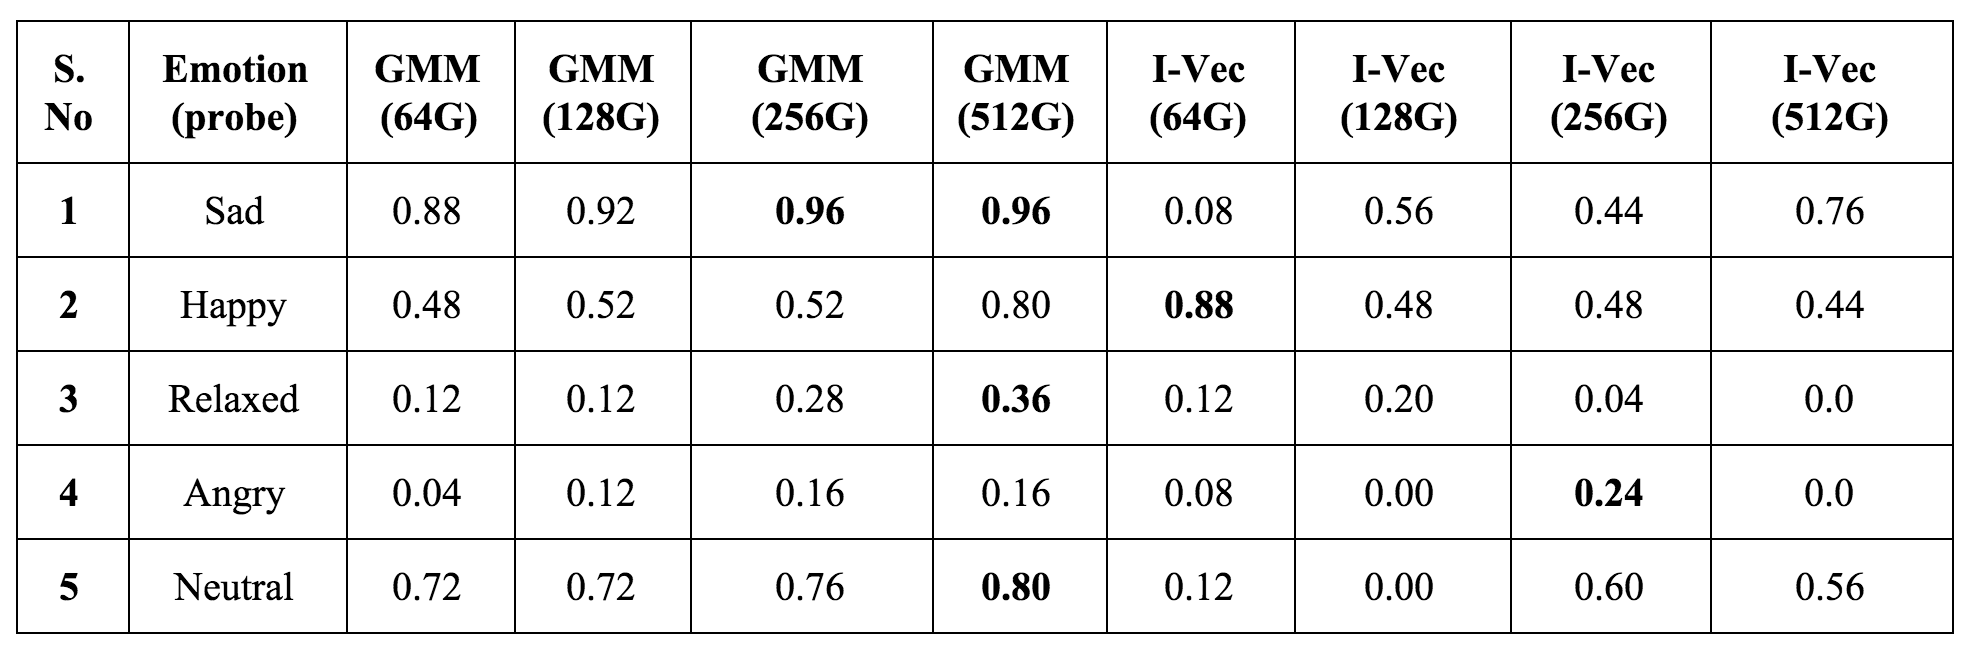
\includegraphics[height=40mm,  width=130mm]{figures/7_25fold.png}
		\caption[Emotion Recognition - Accuracy over 25 fold]{Accuracy: 25 Fold Test Data:  GMM vs I - Vector}
			\label{25fold}
\end{figure}
	
	\subsection{Experiments}
	As indicated, we have divided our test data into several folds and then run experiments based on trained GMM-UBM and I-Vector Models. The UBM of choice is Giant UBM (TIMIT UBM + FAU (non-emotion labeled)). The dimension of MFCC chosen was: 39. The number of test folds: 25, 50, 100 and 250. And number of Gaussian chosen was 64, 128, 256 and 512. We show the accuracy results for all the experiments in figures \ref{25fold}, \ref{50fold}, \ref{100fold} and \ref{250fold}  and highlight the best score for each emotion probe.
 	\subsection{Observations and Results: GMM vs I-Vectors}
\begin{figure}[ht!]
	\centering
		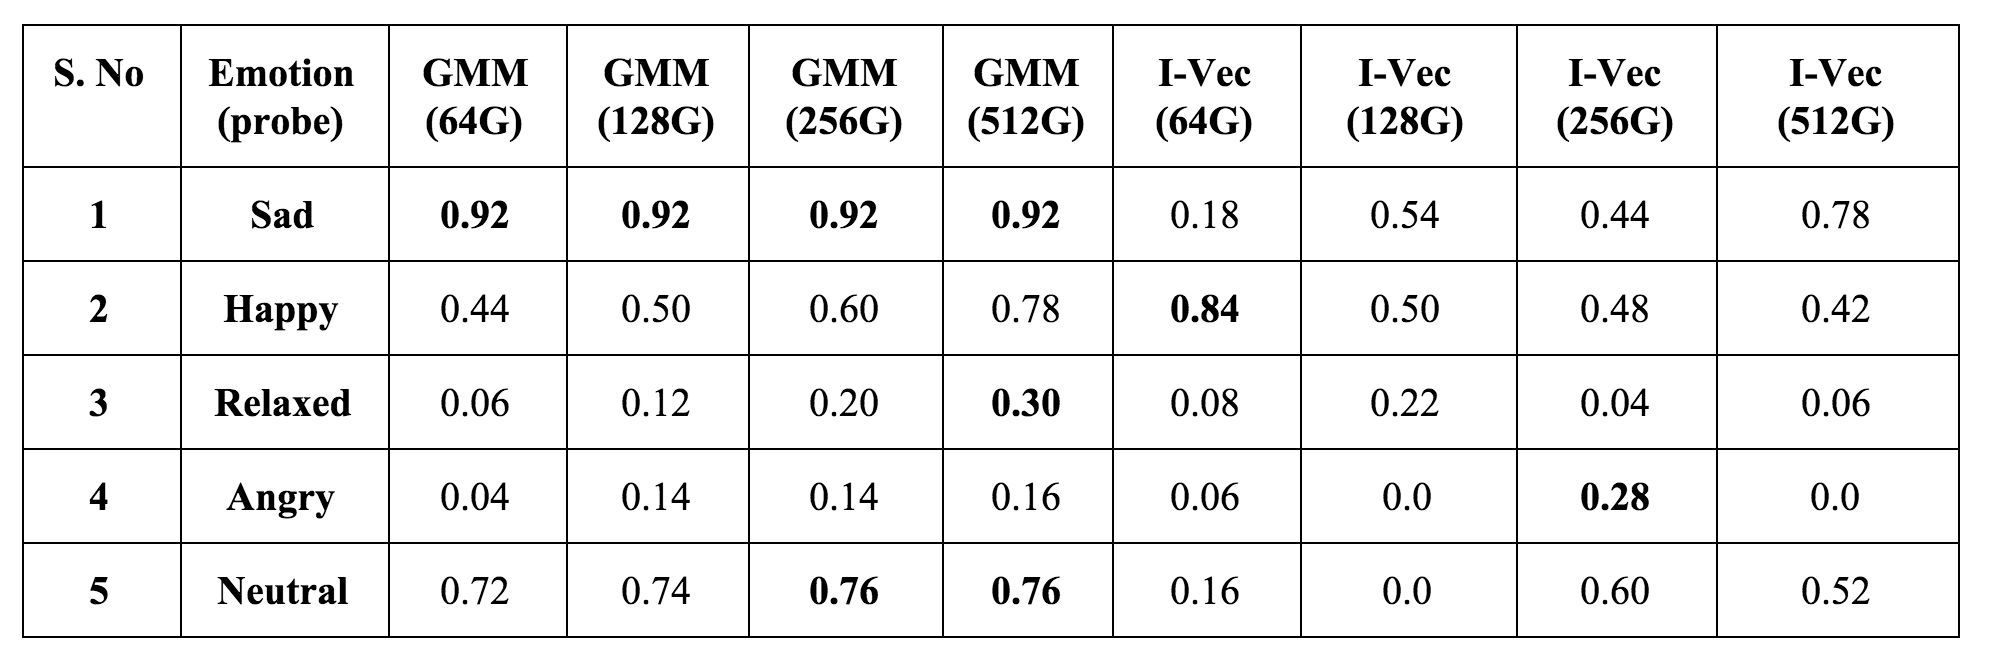
\includegraphics[height=40mm,  width=130mm]{figures/7_50fold.png}
		\caption[Emotion Recognition - Accuracy over 50 fold]{Accuracy: 50 Fold Test Data:  GMM VS vs I - Vector}
			\label{50fold}
\end{figure}

\begin{figure}[ht!]
	\centering
		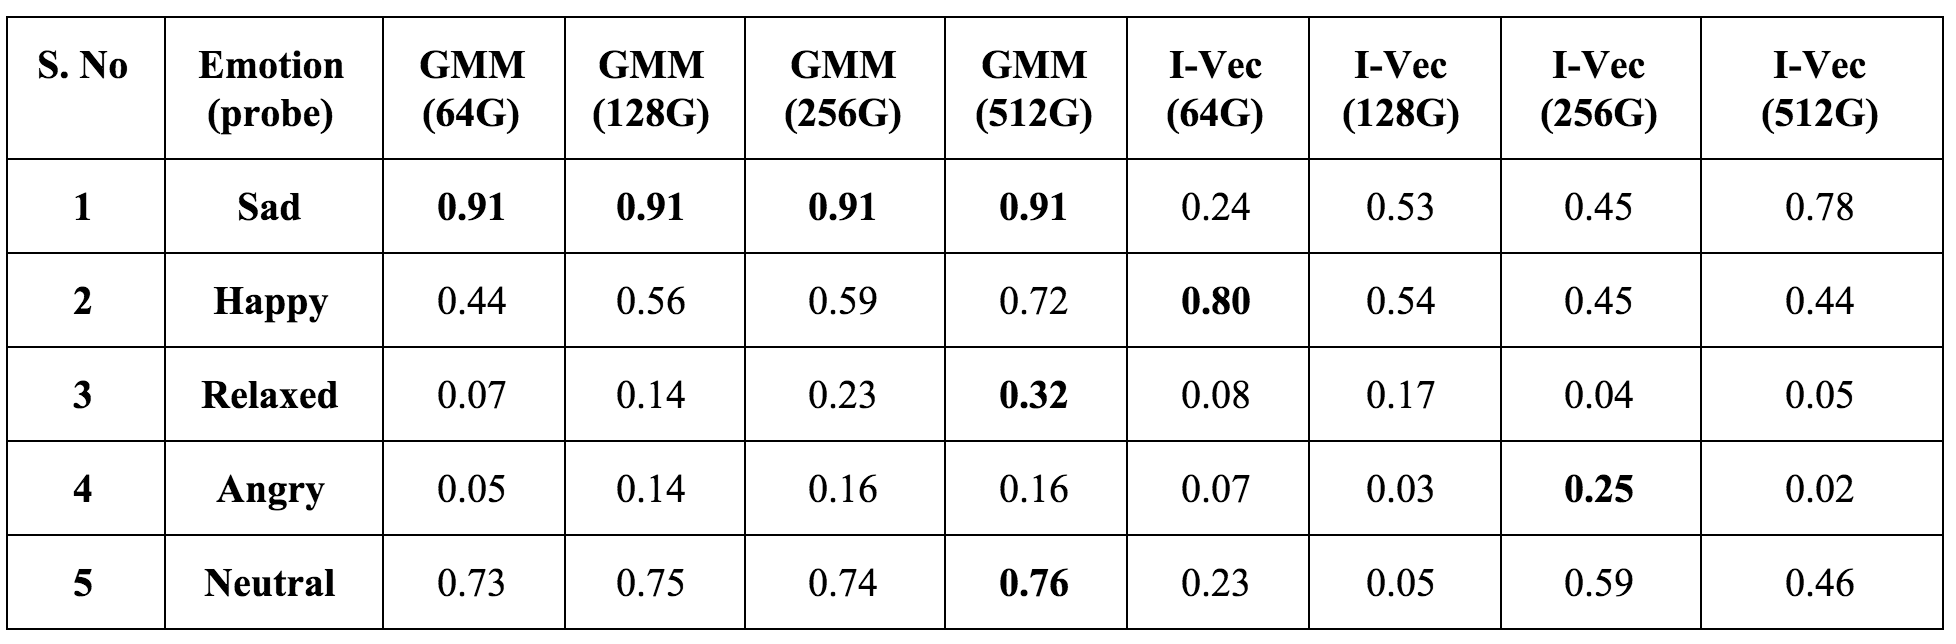
\includegraphics[height=40mm,  width=130mm]{figures/7_100fold.png}
		\caption[Emotion Recognition - Accuracy over 100 fold]{Accuracy: 100 Fold Test Data:  GMM vs I - Vector}
			\label{100fold}
\end{figure}

\begin{figure}[ht!]
	\centering
		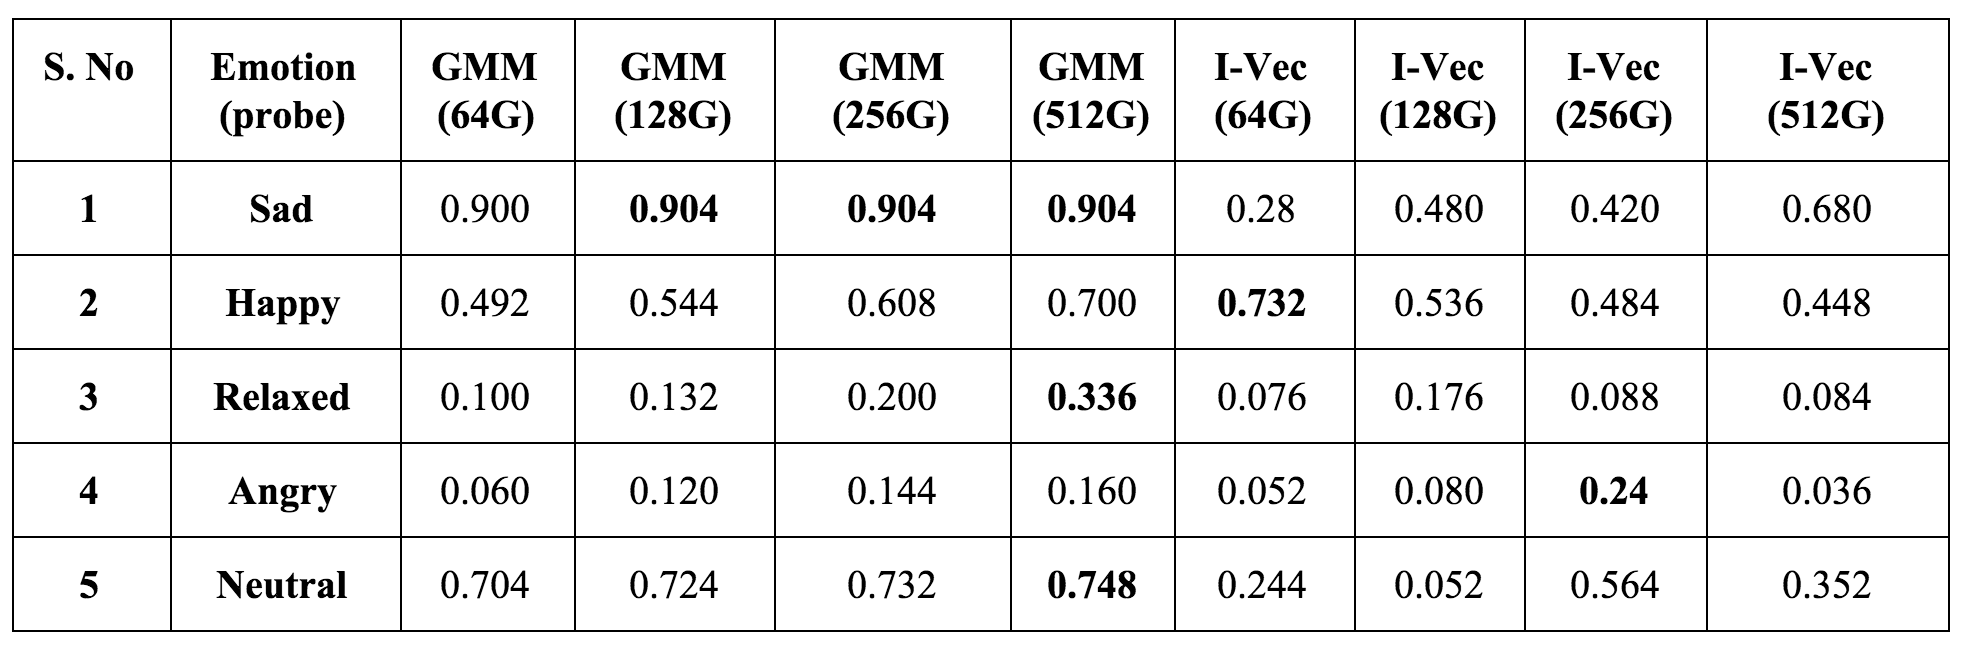
\includegraphics[height=40mm,  width=130mm]{figures/7_250fold.png}
		\caption[Emotion Recognition - Accuracy over 250 fold]{Accuracy: 250 Fold Test Data:  GMM vs I - Vector}
			\label{250fold}
\end{figure}

We clearly indicate in figures  \ref{25fold}, \ref{50fold}, \ref{100fold} and \ref{250fold} that for the Semaine dataset, GMM method outperforms the I - Vector methods for all emotion categories except class “Angry”, which is around 28% and class “Happy”, which is around 88%  as the best result for I-Vectors. We also found that the number of Gaussians play a pivotal role in gathering accuracies. When the number of gaussians was chosen as 512, the best results were obtained overall.  Moreover, 512 GMM seems to perform the best, as it clearly gives the best result for sad, relaxed and neutral categories. 


\begin{figure}[ht!]
	\centering
\subfigure[Best overall accuracy result fold-wise]{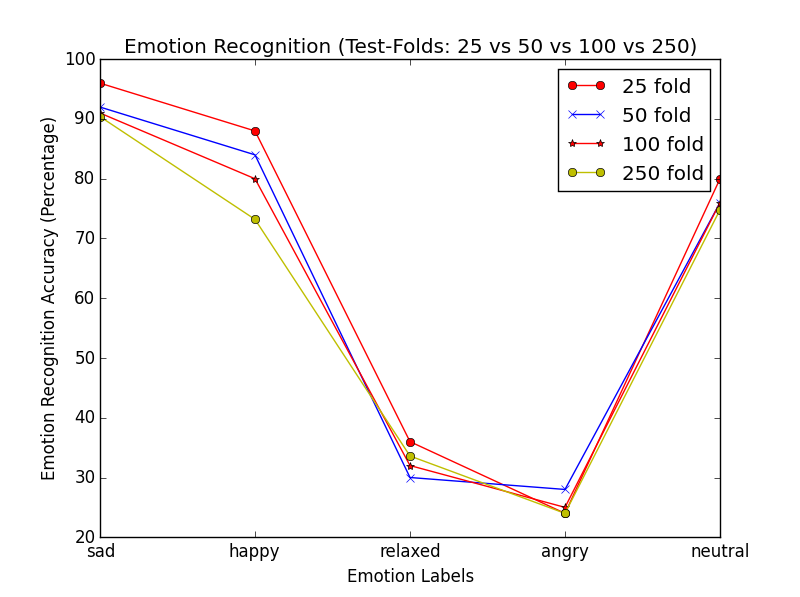
\includegraphics[height=60mm,  width=70mm]{figures/7_plot1.png}\label{plot1}}
\subfigure[Best accuracy result for GMM-UBM vs I-Vector for each fold-wise.]{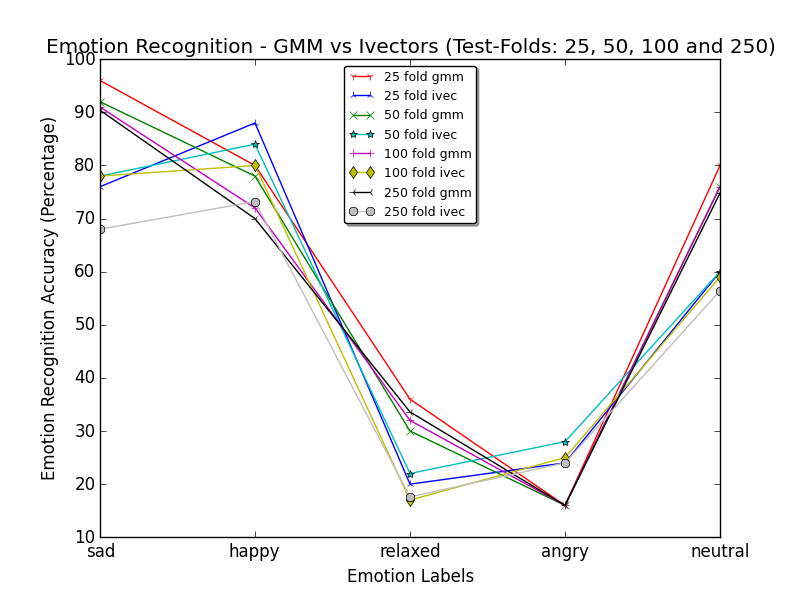
\includegraphics[height=60mm,  width=70mm]{figures/7_plot2.png}\label{plot2}}
\caption{Emotion wise plots for accuracy w.r.t. folds.}
\end{figure}


Closely observing figure ~\ref{plot1} which indicates the best result for each fold, we can see the effects of using the various test fold data on accuracy and conclude that: 25 folds is performing the best. Thus, increasing the number of folds has a rather negative effect. But, this is not true in context of GMM vs I-Vectors since the I-Vectors don’t perform well on low number of folds. We find best I-Vector results for higher number of folds, Figure ~\ref{plot2}. As per observations, 50 fold I-Vector performs the best among all I-Vectors roughly for all emotion classes.

 \section{Deep Neural Networks for Emotion Recognition}
 
 Continuing our journey with application of Deep Learning to text for capturing sentiment, In this section we now move to apply the same idea to emotion recognition. We will only highlight one recent work, by Kun Han et. al, \parencite{deepemotionrecog} who proposed to utilize Deep Neural Networks to extract high level features from raw data and show they are effective for speech emotion recognition. The method supposedly learns exceedingly well the low level features and demonstrates 20\% accuracy over the current state of the art methods. The evaluation was performed upon the Interactive Emotional Dyadi Motion Capture (IEMOCAP) database ~\parencite{iemocap}.  